
\subsection{Fitting problem}
In order to represent a given line or surface by Bezier curves or surfaces respectively, just as with NURBS, one has to solve a fitting problem. The goal of it is to fit in a parametric curve to the set of given data points. In the case of interest, the given set of points is a mesh, obtained from surface contouring.
\subsubsection{Fitting problem: Bezier curve}
First we want to find a Bezier-curve $\vec{B}_n\left(u\right)$ of degree $n$ which is approximating a given spline $\vec{s}_m\left(u\right)$ defined by $m$ points in a optimal way. For this purpose we want to minimize the L2-error. This leads to the minimization problem
\begin{equation}
\text{find\ } \underset{\vec{B}_n\in \mathbb{B}_n}{\min} \Ltwonorm{\vec{B}_n-\vec{s}_m}.
\end{equation}
Minimizing the L2-norm is equal to minimizing the functional:
\begin{equation}
F(\vec{B}_n)=\int\limits_{u=0}^{u=1} \left(\vec{B}_n-\vec{s}_m\right)^2\du
\end{equation}
Using the variational principle we get the the system of linear equations
\begin{equation}
A a = b
\end{equation}
where $A$ is the matrix of pair-wise scalar products of basis functions (Bernstein polynomials), $b$ is the vector of scalar products of the given spline $s_{m}$ and basis functions and $a$ is a required vector of coefficients for Bezier curve representation.

\subsubsection{Fitting problem (least squares): NURBS}
Although the approach used above showed good results, it appears to be very computationally intensive. Analogically, one could reduce the original problem to a \emph{regression problem}, which allows us to reduce computational costs. Also, to improve the locality of our solution, from now on we are going to use NURBS basis functions with weights $\omega_{j} = 1$ instead of Bezier curves. For this purpose, we adopted an algorithm, provided in \cite{becker2011advanced}:

Let $X^{0}$ be the $n \times 2$ matrix of the given set of points, $N^{p}$ the basis functions of degree $p$ ($n \times (n+p)$ matrix, where $n$ is the number of points), and $P^{0}$ the control points ($(n+p) \times 2$ matrix).

The original problem can be written as:
\begin{equation}
X_{i}^{0} = \sum\limits_{j=1}^{n+p} P_{j}^{0} N_{i,j}^{p}, \quad i \in \{1,..,n\}
\end{equation}
Or, in short:
\begin{equation}
X^{0} = N^{p} P^{0}
\end{equation}
The above system needs to be solved for the unknown $P^{0}$. This can be done numerically, for example through singular value decomposition. 
%part of implementation

\subsubsection{Fitting Problem: Peter's Scheme}
\todo[inline]{insert stuff here}

\subsection{Fitting pipeline}
\begin{figure}
\centering
  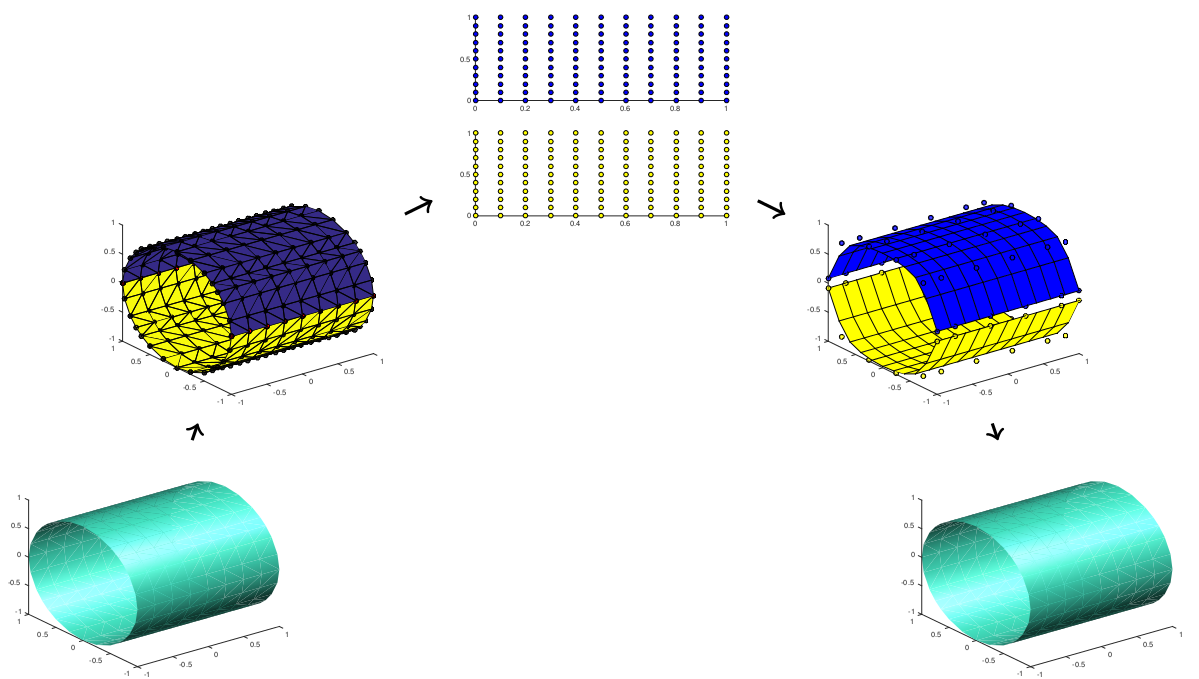
\includegraphics[width=.85\linewidth]{Fitting_workflow.png}
  \caption{NURBS fitting pipeline}
  \label{fig:fitting_pipeline}
\end{figure}
Since the geometry obtained after topology optimization can be arbitrary complex, we might not be able to find a good fit using only one patch. We seek a multi step algorithm, allowing us to break the overall big problem into smaller problems, which can be handled relatively easy.
Based on the algorithm described in \cite{eck1996automatic}, our overall fitting pipeline looks as follows (see \autoref{fig:fitting_pipeline}):
\begin{itemize}
	\item Patch selection (breaking our problem in small pieces which can be solved using least squares)
	\item Parametrization of obtained patches
	\item B-spline fitting using least squares
	\item Smooth connection of patches
	\item Conversion back to CAD
\end{itemize}

The pipeline given above, once implemented, will provide us with a flexible algorithm for converting an arbitrary complex mesh based geometry into NURBS and, hence, CAD-representation.